
\subsection*{1.}

\begin{center}
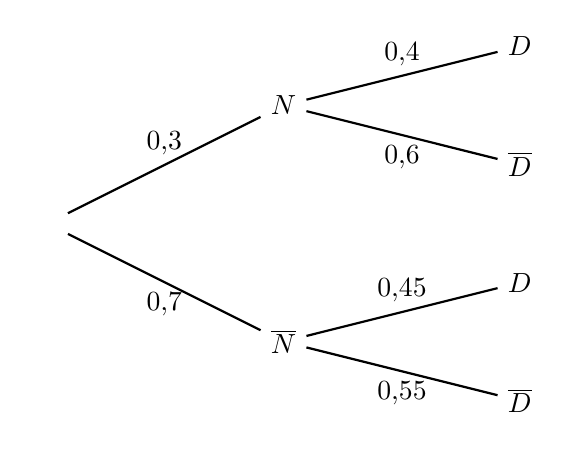
\begin{tikzpicture}[thick, scale=1.5] %{,}
\node (P_-1_0) at (-2,-1.5) {$\phantom{A}$};
\node (P_0_0) at (0,-0.5) {$N$};
\draw (P_-1_0) -- (P_0_0) node[midway, above] {$0{,}3$};
\node (P_1_0) at (2,-0) {$D$};
\draw (P_0_0) -- (P_1_0) node[midway, above] {$0{,}4$};
\node (P_1_1) at (2,-1) {$\overline{D}$};
\draw (P_0_0) -- (P_1_1) node[midway, below] {$0{,}6$};
\node (P_0_2) at (0,-2.5) {$\overline{N}$};
\draw (P_-1_0) -- (P_0_2) node[midway, below] {$0{,}7$};
\node (P_1_2) at (2,-2) {$D$};
\draw (P_0_2) -- (P_1_2) node[midway, above] {$0{,}45$};
\node (P_1_3) at (2,-3) {$\overline{D}$};
\draw (P_0_2) -- (P_1_3) node[midway, below] {$0{,}55$};
\end{tikzpicture}
\end{center}

\subsection*{2.}

Par définition :
\[
p(\overline{N} \cap \overline{D}) = p(\overline{N}) \times p_{\overline{N}}(\overline{D}) = 0{,}7 \times 0{,}55 = 0{,}385.
\]

\subsection*{3.}

On a de même :
\[
p(N \cap \overline{D}) = p(N) \times p_N(\overline{D}) = 0{,}3 \times 0{,}6 = 0{,}18.
\]
D'après la loi des probabilités totales :
\[
p(\overline{D}) = p(N \cap \overline{D}) + p(\overline{N} \cap \overline{D}) = 0{,}18 + 0{,}385 = 0{,}565.
\]

\subsection*{4.}

\[
\begin{array}{|c|c|c|c|c|}
\hline
\text{Évènement} & N \cap D & N \cap \overline{D} & \overline{N} \cap D & \overline{N} \cap \overline{D} \\
\hline
\text{Temps en heure} & 5{,}5 & 6 & 6{,}5 & 7 \\
\hline
\text{Probabilité} & 0{,}12 & 0{,}18 & 0{,}315 & 0{,}385 \\
\hline
\end{array}
\]

Pour la probabilité de l'événement \(\overline{N} \cap D\), on calcule le complément à 1 des trois autres probabilités déjà calculées, soit \(1 - (0{,}12 + 0{,}18 + 0{,}385) = 0{,}315\).

\subsection*{5.}

L'espérance du temps en heure pour le trajet est la somme des produits de chaque temps par leur probabilité, soit :
\begin{align*}
E &= 5{,}5 \times 0{,}12 + 6 \times 0{,}18 + 6{,}5 \times 0{,}315 + 7 \times 0{,}385 \\
&= 0{,}66 + 1{,}08 + 2{,}0475 + 2{,}695 \\
&= 6{,}4825,
\end{align*}
soit un peu moins de 6 h 30 min (en fait à peu près 29 min).

